\section{1174079 - Chandra Kirana Poetra}
\subsection{Teori}
\subsubsection{Kenapa file teks harus di lakukan tokenizer}
\hfill\break
Karena tokenizer berguna untuk memproses atau memisahkan bagian bagian pada teks menjadi beberapa bagian, seperti kalimat atau kata. tokenizer bekerja dengan cara memisahkan kata berdasarkan spasi dan tanda baca
\begin{figure}[H]
\centering
	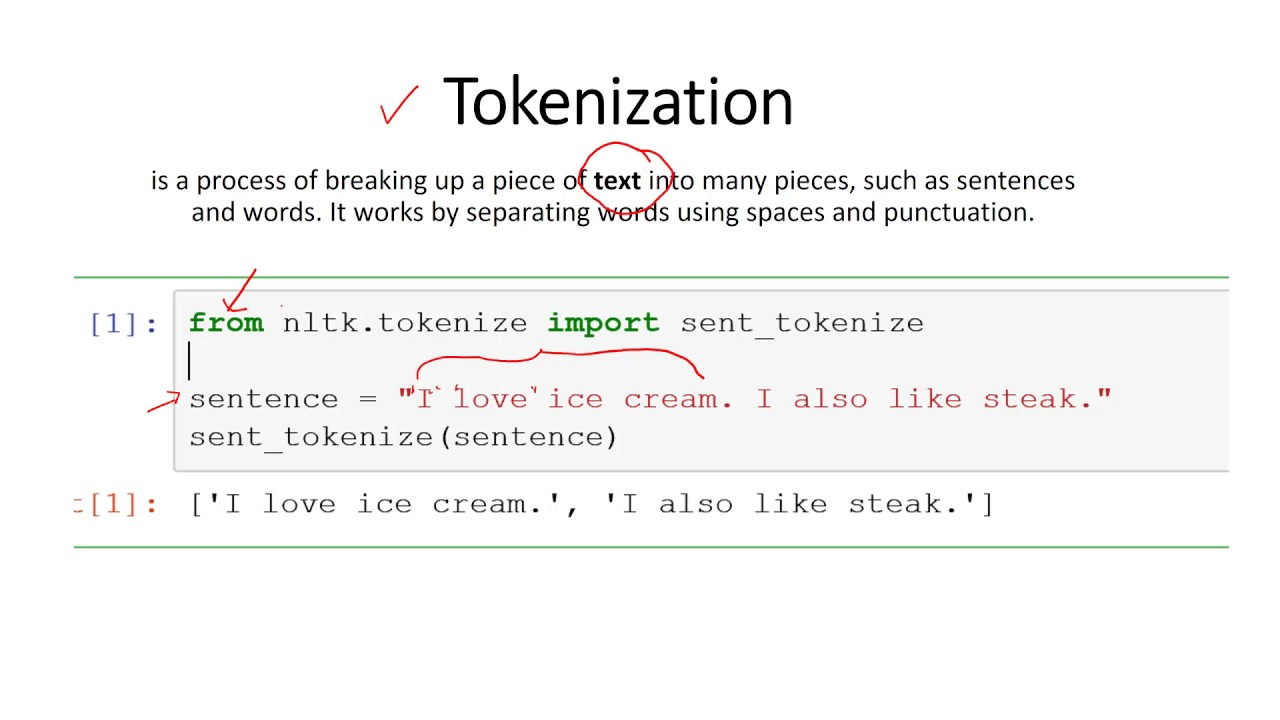
\includegraphics[width=4cm]{figures/1174079/7/token.jpg}
\caption{Teori 1}
\end{figure}

\subsubsection{konsep dasar K Fold Cross Validation pada dataset komentar Youtube pada kode listing 7.1.}
\hfill\break
Konsep sederhana dari K Fold Cross Validation ialah Pada code ini:
\lstinputlisting[firstline=12, lastline=13]{src/1174079/7/1.py}
Kfold diatas bertujuan untuk membagi data kedalam 5 bagian yang nantinya akan menampung komentar dari youtube. data yang dibagi ini nanti akan dihitung dan akan menghasilkan presentase yang bisa dibilang cukup baik
\begin{figure}[H]
\centering
	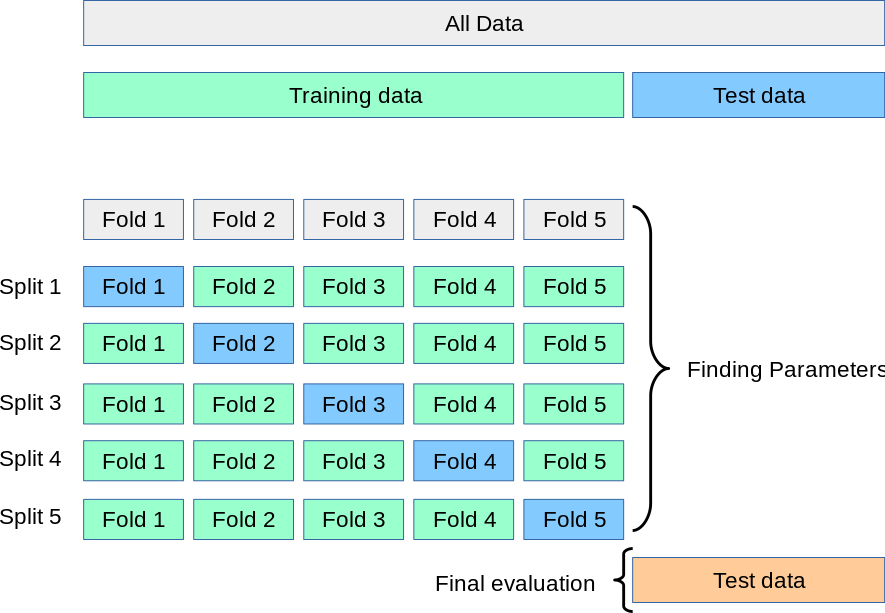
\includegraphics[width=4cm]{figures/1174079/7/kfold.png}
\caption{Teori 2}
\end{figure}

\subsubsection{Apa maksudnya kode program for train, test in splits}
\hfill\break
Data for train adalah data training set, data ini adalah data yang akan kita uji, sementara test in splits adalah data yang akan kita gunakan untuk validasi data training set, keduanya kemudian dibandingkan dan menghasilkan suatu presentase.
\begin{figure}[H]
\centering
	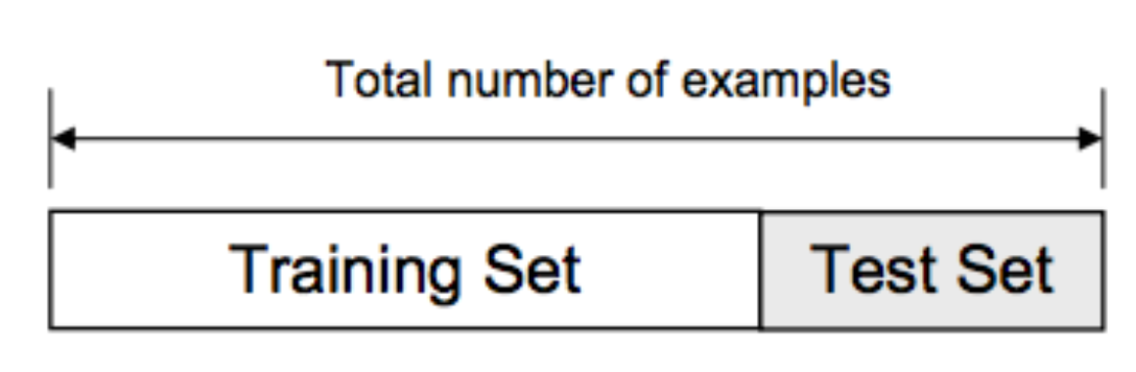
\includegraphics[width=4cm]{figures/1174079/7/trainingset.png}
\caption{Teori 3}
\end{figure}

\subsubsection{Apa maksudnya kode program train content = d[’CONTENT’].iloc[train idx] dan test content = d[’CONTENT’].iloc[test idx]}
\hfill\break
Fungsi dalam kode tersebut berfungsi untuk mengambil data pada kolom atau index CONTENT yang merupakan bagian dari train\_idx dan test\_idx. Contoh sederhananya ketika data telah diubah menjadi data train dan data test maka kita dapat memilihnya untuk ditampilkan pada kolom yang di inginkan. 
\lstinputlisting[firstline=15, lastline=21]{src/1174079/7/1.py}
\begin{figure}[H]
\centering
	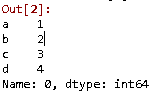
\includegraphics[width=4cm]{figures/1174079/7/nomor3.PNG}
\caption{Teori 4}
\end{figure}

\subsubsection{Apa maksud dari fungsi tokenizer = Tokenizer(num words=2000) dan tokenizer.fit on texts(train content)}
\hfill\break
Berfungsi untuk melakukan proses vektorisasi data menjadi token sebanyak 2000 kata
\begin{figure}[H]
\centering
	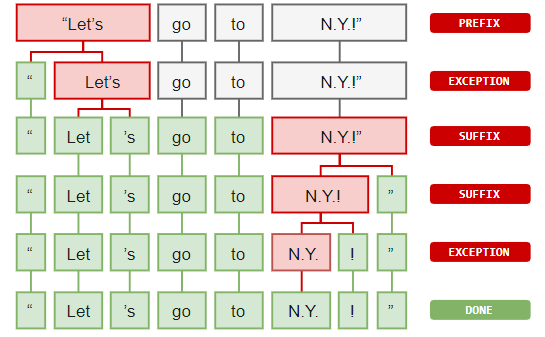
\includegraphics[width=4cm]{figures/1174079/7/fungsitokenizer.png}
\caption{Teori 5}
\end{figure}

\subsubsection{Apa maksud dari fungsi d train inputs = tokenizer.texts to matrix(train content, mode=’tfidf ’) dan d test inputs = tokenizer.texts to matrix(test content, mode=’tfidf ’)}
\hfill\break
Memasukan teks kedalam suatu matrix dengan menggunakan metode TFIDF dan memasukan data testing yang akan diterjemahkan ke suatu matriks
\begin{figure}[H]
\centering
	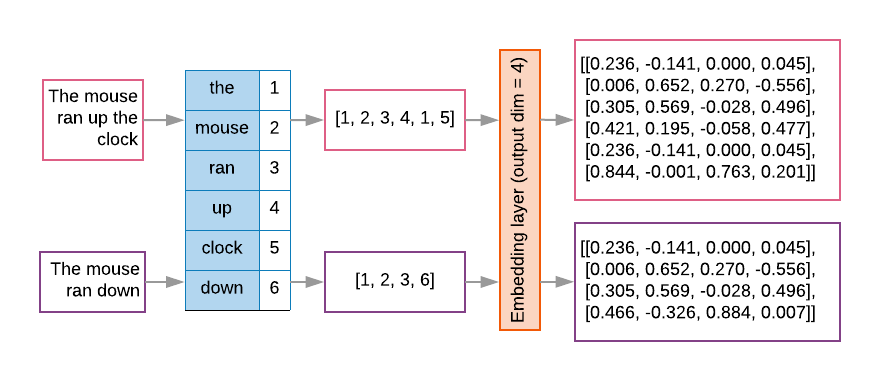
\includegraphics[width=4cm]{figures/1174079/7/EmbeddingLayer.png}
\caption{Teori 6}
\end{figure}

\subsubsection{Apa maksud dari fungsi d train inputs = d train inputs/np.amax(np.absolute(d train inputs)) dan d test inputs = d test inputs/np.amax(np.absolute(d test inputs))}
\hfill\break
Fungsi np.amax digunakan untuk mencari nilai maksimal dari suatu array Jika array tidak ada sumbunya, hasilnya adalah nilai skalar. Jika sumbu diberikan, hasilnya adalah array dimensi a.ndim - 1.
\begin{figure}[H]
\centering
	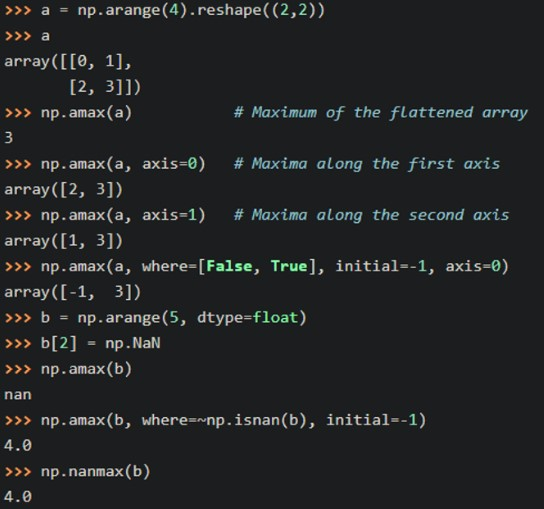
\includegraphics[width=4cm]{figures/1174079/7/7.jpg}
\caption{Teori 7}
\end{figure}

\subsubsection{Apa maksud fungsi dari d train outputs = np utils.to categorical(d[’CLASS’].iloc[train idx]) dan d test outputs = np utils.to categorical(d[’CLASS’].iloc[test idx]) dalam kode program}
\hfill\break
Membuat variable dengan nama train outputs yang diisi dengan kategori dari class dengan menggunakan ketentuan iloc train idx. Kemudian menampungnya.
\begin{figure}[H]
\centering
	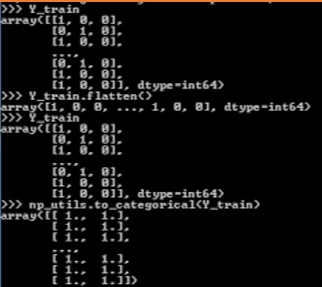
\includegraphics[width=4cm]{figures/1174079/7/8.jpg}
\caption{Teori 8}
\end{figure}

\subsubsection{Apa maksud dari fungsi di listing 7.2.}
\hfill\break
\lstinputlisting[firstline=26, lastline=31]{src/1174079/7/1.py}
Fungsinya adalah model perlu mengetahui jenis data input apa yang digunakan atau yang seharusnya. Oleh karena itu, lapisan pertama adalah model Sequential (Karena model sequential ini dapat mengerjakan inferensi secara otomatis) perlu menerima informasi tentang bentuk inputnya.
\begin{figure}[H]
\centering
	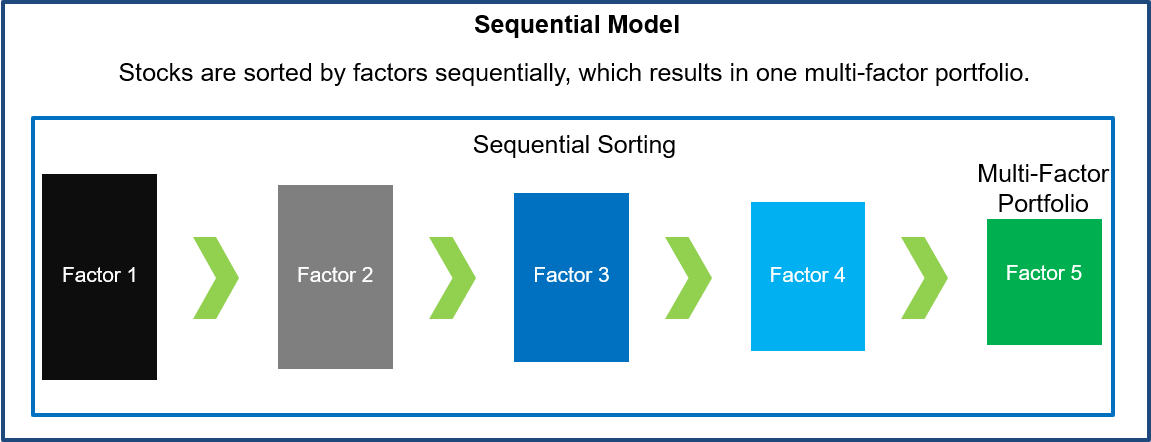
\includegraphics[width=4cm]{figures/1174079/7/sequentialmodel.png}
\caption{Teori 9}
\end{figure}

\subsubsection{Apa maksud dari fungsi di listing 7.3 dengan parameter tersebut}
\hfill\break
\lstinputlisting[firstline=34, lastline=35]{src/1174079/7/1.py}
Kode diatas merupakan fungsi yang digunakan untuk mendefinisikan loss function, optimizer, dan juga metrics yang akan digunakan pada data yang akan kita train. categoricalcrossentropy merupakan function loss yang kita gunakan untuk melakukan perhitungan, sementara optimizer yang kita gunakan adalah adam, selain adam, ada juga SGD,RMSprop, dan lain lain dan metrics accuracy adalah value yang akan kita cari nilainya
\begin{figure}[H]
\centering
	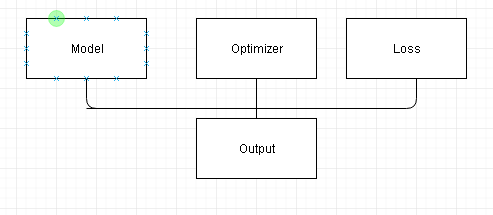
\includegraphics[width=4cm]{figures/1174079/7/modelcompile.PNG}
\caption{Teori 10}
\end{figure}

\subsubsection{Apa itu Deep Learning}
\hfill\break
Merupakan cabang dari machine learning yang berasal dari cabang lainnya yaitu artificial intelligence,  deep learning mempunyai kemampuan jaringan pembelajaran dengan metode unsupervised dari data yang tidak ada strukturnya maupun tidak ada label yang dikenal juga sebagai deep neural network
\begin{figure}[H]
\centering
	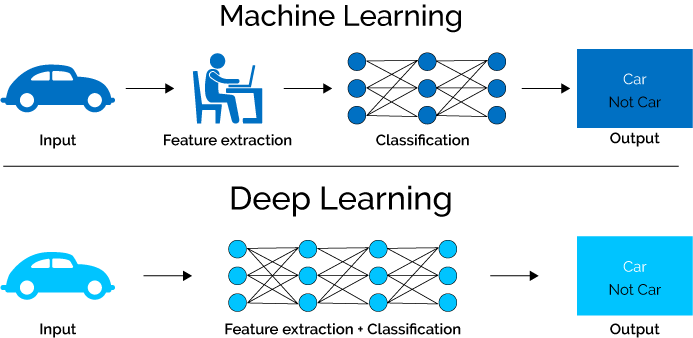
\includegraphics[width=4cm]{figures/1174079/7/DeepLearning.png}
\end{figure}

\subsubsection{Apa itu Deep Neural Network, dan apa bedanya dengan Deep Learning}
\hfill\break
Komponen Neural netwrok adalah neuron yang dilabeli sebagai j yang menerima input dari neuron sebelumnya, seringkali dalam bentuk fungsi identifikasi untuk menyediakan output, sementara deep learning menggunakan motherboard, processor, ram, dan cpu untuk melakukan prosesnya

Neural netwrok menggunakan metode feed forward neural network atau bisa juga recurent network sementara deep learning menggunakan unsupervised pretrained network atau convulutional neural network

\subsubsection{Jelaskan dengan ilustrasi gambar buatan sendiri(langkah per langkah) bagaimana perhitungan algoritma konvolusi dengan ukuran stride (NPM mod3+1) x (NPM mod3+1) yang terdapat max pooling.}	
\hfill\break
Algoritma Konvolusi  merupakan suatu algoritma yang dapat memproses gambar yang nantinya digunakan untuk membedakan satu gambar dengan yang lainnya, strides merupakan salah satu parameter yang ada, yang digunakan untuk mendefinisikan jumlah pergerakan pixel pada input matrix, ketika didefinisikan 1 stridenya, maka satu pixels akan pindah dalam satu waktu, jika 2 maka dua pixel akan pindah secara bersamaan dalam satu waktu
\begin{figure}[H]
\centering
	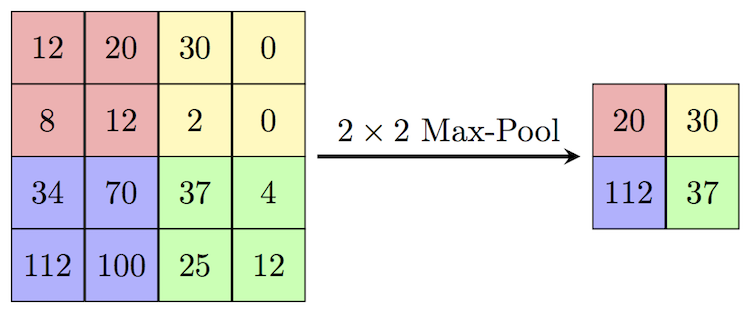
\includegraphics[width=4cm]{figures/1174079/7/MaxpoolSample.png}
\caption{Teori 11}
\end{figure}



\subsection{Praktek}
\subsubsection{Nomor 1}
\hfill\break
\lstinputlisting[firstline=9, lastline=11]{src/1174079/7/2.py}


\subsubsection{Nomor 2}
\hfill\break
\lstinputlisting[firstline=14, lastline=27]{src/1174079/7/2.py}


\subsubsection{Nomor 3}
\hfill\break
\lstinputlisting[firstline=30, lastline=34]{src/1174079/7/2.py}


\subsubsection{Nomor 4}
\hfill\break
\lstinputlisting[firstline=37, lastline=41]{src/1174079/7/2.py}


\subsubsection{Nomor 5}
\hfill\break
\lstinputlisting[firstline=44, lastline=45]{src/1174079/7/2.py}


\subsubsection{Nomor 6}
\hfill\break
\lstinputlisting[firstline=48, lastline=49]{src/1174079/7/2.py}


\subsubsection{Nomor 7}
\hfill\break
\lstinputlisting[firstline=52, lastline=54]{src/1174079/7/2.py}


\subsubsection{Nomor 8}
\hfill\break
\lstinputlisting[firstline=57, lastline=62]{src/1174079/7/2.py}


\subsubsection{Nomor 9}
\hfill\break
\lstinputlisting[firstline=65, lastline=67]{src/1174079/7/2.py}


\subsubsection{Nomor 10}
\hfill\break
\lstinputlisting[firstline=71, lastline=83]{src/1174079/7/2.py}


\subsubsection{Nomor 11}
\hfill\break
\lstinputlisting[firstline=86, lastline=87]{src/1174079/7/2.py}


\subsubsection{Nomor 12}
\hfill\break
\lstinputlisting[firstline=90, lastline=99]{src/1174079/7/2.py}


\subsubsection{Nomor 13}
\hfill\break
\lstinputlisting[firstline=102, lastline=130]{src/1174079/7/2.py}


\subsubsection{Nomor 14}
\hfill\break
\lstinputlisting[firstline=133, lastline=143]{src/1174079/7/2.py}


\subsubsection{Nomor 15}
\hfill\break
\lstinputlisting[firstline=146, lastline=148]{src/1174079/7/2.py}


\subsubsection{Nomor 16}
\hfill\break
\lstinputlisting[firstline=151, lastline=151]{src/1174079/7/2.py}


\subsubsection{Nomor 17}
\hfill\break
\lstinputlisting[firstline=154, lastline=154]{src/1174079/7/2.py}

\subsubsection{Nomor 18}
\hfill\break
\lstinputlisting[firstline=158, lastline=160]{src/1174079/7/2.py}


\subsubsection{Nomor 19}
\hfill\break
\lstinputlisting[firstline=163, lastline=174]{src/1174079/7/2.py}


\subsubsection{Nomor 20}
\hfill\break
\lstinputlisting[firstline=177, lastline=179]{src/1174079/7/2.py}

\subsection{Penanganan Error}
\subsubsection{Error}
\hfill\break
\begin{itemize}
\item NameError

\begin{figure}[H]
\centering
	
\includegraphics[width=4cm]{figures/1174079/7/error.PNG}
\caption{NameError}
\end{figure}
\end{itemize}
\subsubsection{Solusi Error}
\hfill\break
\begin{itemize}
\item NameError

Pastikan sudah diimport atau cek typo
\end{itemize}

\subsection{Bukti Tidak Plagiat}
\begin{figure}[H]
	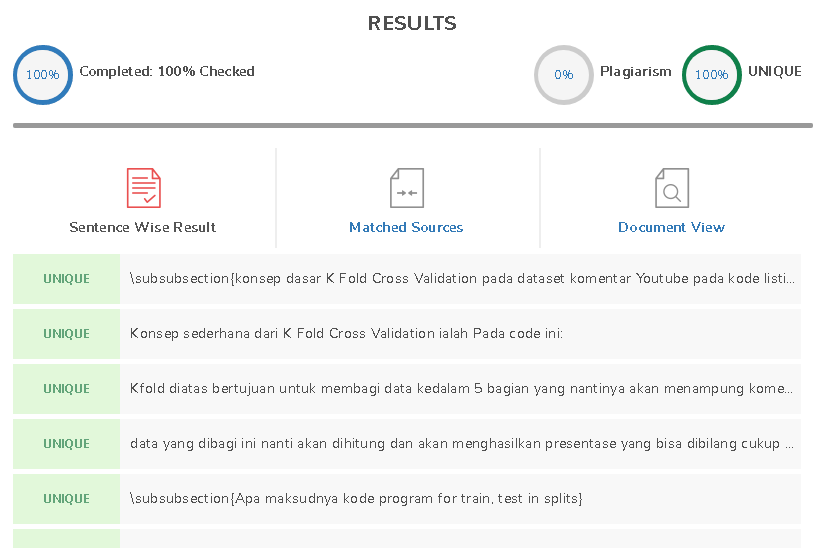
\includegraphics[width=4cm]{figures/1174079/7/plagiat.PNG}
	\centering
	\caption{Bukti tidak plagiat}
\end{figure}

\subsection{Link Youtube}
https://youtu.be/AHJOIZJYd9I